\section{Simple measures of responsiveness}
\label{sec:responsiveness}

\subsection{Thresholding $|U_{10}|^2$ responsiveness}
\label{sec:thresh-resp}

As shown in Figure~19~of~T20~\cite{ZannaPreprint} (see Figure~\ref{fig:yin-responsiveness}).
The threshold seems arbitrary,
so I chose that the $\Delta\eta_{\mathrm{hp}} \ge 0$ (Figure~\ref{fig:simple-responsiveness-results}),
as it approximately guarantees that the sea surface stress is acting into
the coast.


\subsection{$\tau_u$, $\tau_v$ responsiveness}
\label{sec:tau-tau}
This method is quite crude, and could be simply improved.
Figure~\ref{fig:tau-tau-r-no} shows a single example of working out the linear
responsiveness in \texttt{tyr}, which is applied along \texttt{eUS} in
Figure~\ref{fig:tau-tau-resp}.
Figure~\ref{fig:tau-tau-responsiveness}
creates a more robust metric for the responsiveness.

\begin{figure}
\centering
\includegraphics[width=1\linewidth]{../surge/plots/3d_plots/3d_plotnorlean.pdf}
 \caption{New Orleans \texttt{tyr} fit for 2005 (red) and 2004 (blue) using
 \texttt{huber}, \texttt{MLR}, \texttt{RANSAC} and \texttt{Theil-Sun}~\cite{scikit-learn}.
 \texttt{huber} and \texttt{MLR} are the most reliable, so are used further in later
 sections.}
 \label{fig:tau-tau-r-no}
\end{figure}


\begin{figure*}[htb!]
    \centering
    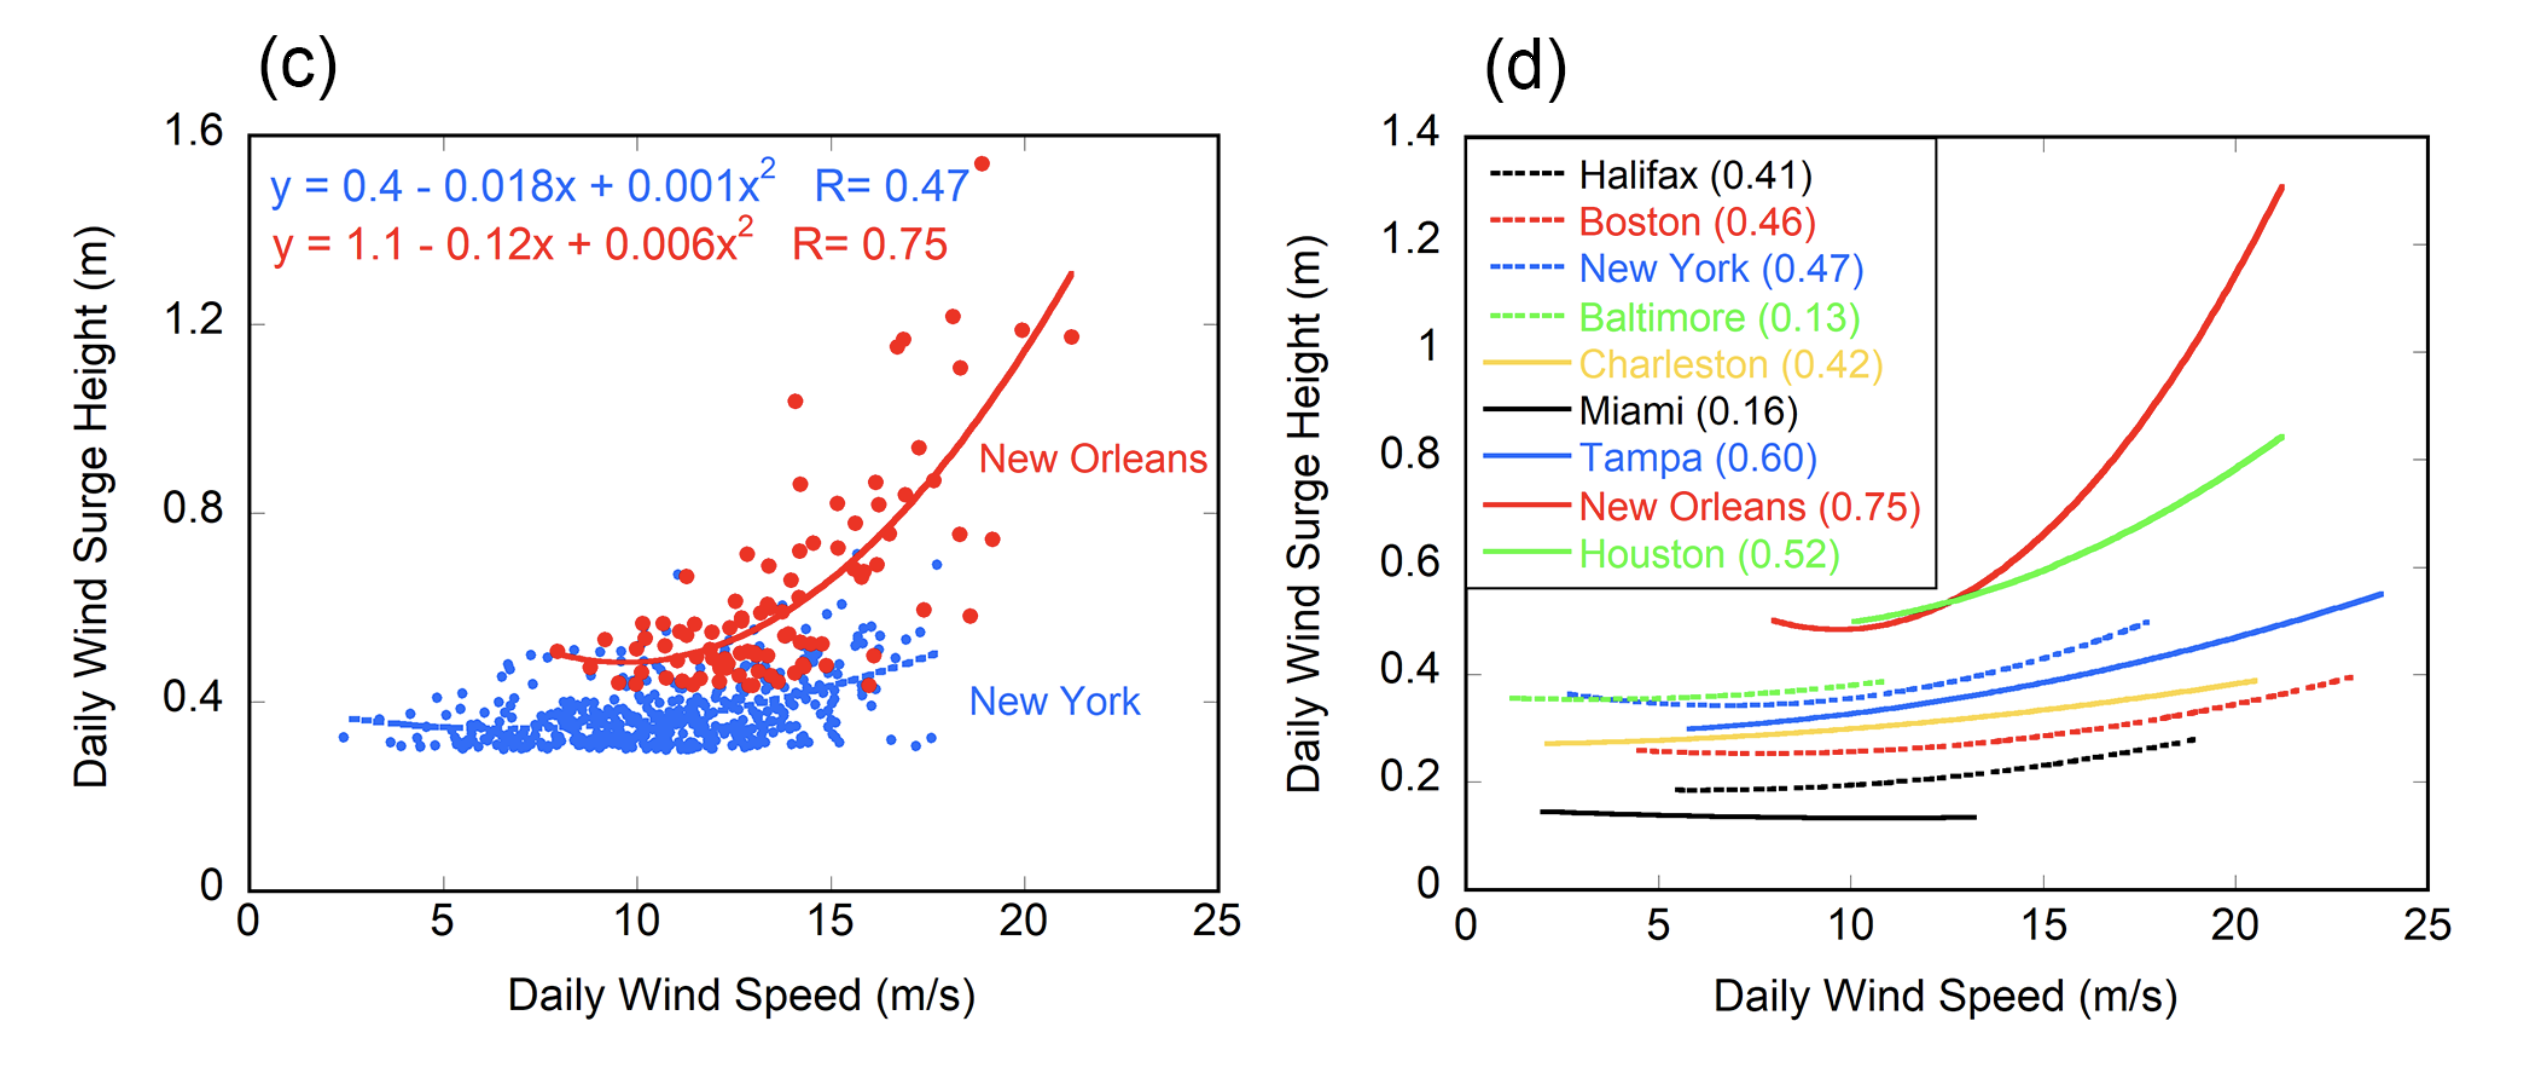
\includegraphics[width=0.8\linewidth]{images/example-images/yin-responsiveness.png}
    \vspace{-7pt}
    \caption{Figure 10c \& 10d in Yin et al.~2020~\cite{ZannaPreprint}. }
   \label{fig:yin-responsiveness}

   \includegraphics[width=0.8\linewidth]{../surge/plots/score-plot/score_plot.pdf}
   \vspace{-7pt}
   \caption{Linear Regression of $ \Delta \eta$ against $|U|^2$ for $ \Delta\eta>0$.
   Only generalises for the most vulnerable points. Most variance not modelled.}
  \label{fig:simple-responsiveness-results}
\end{figure*}




\begin{figure*}
\centering
 \hspace{-40pt} \includegraphics[width=0.6\linewidth]{../surge/plots/rmlr.pdf}
  \vspace{-15pt}
 \caption{A four panel plot to show the estimation of responsiveness
          of $\Delta\eta_{\mathrm{hp}}$ to $\tau_u$ and $\tau_v$, with the
          \texttt{MLR} and \texttt{Huber} algorithms. The y-units of A~\&~B are
           m Pa$^{-1}$.}
 \label{fig:tau-tau-resp}
 \hspace{-40pt} \includegraphics[width=0.3\linewidth]{../surge/plots/reg_angle.png}
  \vspace{-15pt}
 \caption{This shows that for the majority of the coastline there is a close
 corresponce between the normal bearing of the coast and the regression line ($r_p=0.83\pm0.05$).
 \texttt{np.arctan2(c0, c1)}}
  \label{fig:tau-tau-angle}
  \hspace{-40pt} \includegraphics[width=0.5\linewidth]{../surge/plots/adj_reg_mag.pdf}
   \vspace{-15pt}
  \caption{A more robust measure of responsiveness magnitude.
  ($\bar{r^2}$)\texttt{*np.sqrt(np.square(c0) + np.square(c1))}. }
   \label{fig:tau-tau-responsiveness}
\end{figure*}


\label{sec:angle}

Figure~\ref{fig:tau-tau-angle} shows that the angle is highly correlated with
the bearing of the coast (see~§~\ref{sec:convexity}).
This bearing is compared to the normal coastline bearing).
As shown in Figure~\ref{fig:tau-tau-angle}, there is a systematic offset between the two lines,
with a slight change between them, which can be explained through
 Ekman transport~\cite{hope2013hindcast}.


\label{sec:reg-metrics}

The magnitude of this regression line varies in approximately the same
way for both\footnote{QUANTIFY!!} (Figures~\ref{fig:simple-responsiveness-results},~\ref{fig:tau-tau-resp}~\&~\ref{fig:tau-tau-responsiveness}),
showing that there is some underlying property of the
coastline that both illuminate.
Figure~\ref{fig:learnt-eus}, uses lasso and ridge regression to
estimate the relationship between the coastal metrics (§~\ref{sec:convexity}~\&~\ref{sec:bath-grad})
and either responsiveness metric.
It is possible that this is a spurious structure, where the fit
is made possible by giving so many information-less channels to fit against.
We use \texttt{vc} and \texttt{jap} as in Figure~\ref{fig:learnt-vc},
to check that this generalises.

\label{sec:generalisability}


\begin{figure}[htb!]
    \centering
    \includegraphics[width=0.7\linewidth]{../surge/plots/ridge_lasso.pdf}
    \vspace{-15pt}
   \caption{\texttt{eUS} regression learning.
    Although not for lasso, and the regression is not consistent.
            We also need another coast to see if this generalises.}
    \label{fig:learnt-eus}

    \centering
    \includegraphics[width=0.8\linewidth]{../surge/plots/vc_ridge_lasso.pdf}
    \caption{The same as above, but for the \texttt{vc} coastline.}
    \label{fig:learnt-vc}
\end{figure}




\FloatBarrier
